% Part: model-theory
% Chapter: interpolation
% Section: separation

\documentclass[../../../include/open-logic-section]{subfiles}

\begin{document}

\olfileid[hi]{mod}{int}{sep}

\olsection{\printtoken{P}{sentence} का पृथक्करण}

अंतर्वेशन प्रमेय के प्रमाण पर आगे बढ़ने से पहले कुछ आधार तैयार करना
आवश्यक है। $!A$ और $!B$ का अंतर्वेशक ऐसा !!a{sentence}~$!C$ है कि
$!A \Entails !C$ और $!C \Entails !B$। प्रतिपक्ष द्वारा, बाद वाला कथन
तभी और केवल तभी सत्य है जब $\lnot !B \Entails \lnot
!C$। इस गुण वाले
!!^a{sentence}~$!C$ को $!A$ और $\lnot !B$ को \emph{पृथक करने वाला}
कहते हैं। अतः $!A$ और $!B$ का अंतर्वेशक खोजना, $!A$ और $\lnot !B$ को
पृथक करने वाला !!a{sentence} खोजने के बराबर है। जैसा प्रायः होता है,
एक व्यापकीकरण पर विचार करना उपयोगी होगा: ऐसा वाक्य जो !!{sentence}s के
दो \emph{समुच्चयों} को पृथक करे।

\begin{defn}
कोई वाक्य $!C$, वाक्यों के समुच्चयों $\Gamma$ और $\Delta$ को तभी और केवल
तभी \emph{पृथक करता है} जब $\Gamma \Entails !C$ और $\Delta \Entails
\lnot !C$। यदि ऐसा कोई !!{sentence} नहीं है, तो $\Gamma$ और $\Delta$
\emph{अपृथक्करणीय} हैं।
\end{defn}

$\Gamma$, $\Delta$ और $!C$ के प्रतिरूपों के वर्गों के बीच समावेशन-संबंध
नीचे दर्शाए गए हैं:
\begin{figure}[h]
  \centering
  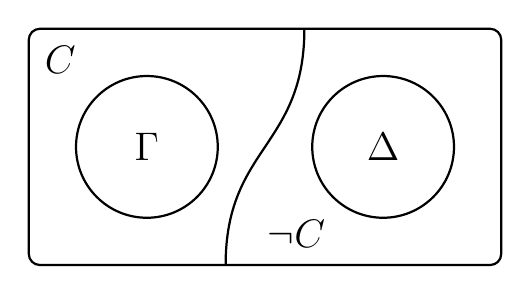
\begin{tikzpicture}[node distance=2cm, auto, thick]
    \draw [rounded corners] (0,0) -- (6,0) -- (6,3) -- (0,3) --  cycle;
    \draw (1.5,1.5) circle (0.9cm);
    \draw (4.5,1.5) circle (0.9cm);
    \path node at (1.5,1.5) {\Large $\Gamma$}; 
    \path node at (4.5,1.5) {\Large $\Delta$}; 
    \path node at (0.4,2.6) {\Large $\formula{C}$};
    \path node at (3.4,0.4) {\Large $\lnot \formula{C}$};
    \draw (2.5,0) .. controls (2.5,1.5) and (3.5,1.5) .. (3.5,3);
  \end{tikzpicture}
  \caption{$!C$, $\Gamma$ और $\Delta$ को पृथक करता है}
  \ollabel{fig:sep}
\end{figure}


\begin{lem}\ollabel{lem:sep1}
मान लें कि $\Lang{L}_0$ वह भाषा है जिसमें प्रत्येक ऐसा !!{constant},
!!{function} और !!{predicate} ($\doteq$ के अतिरिक्त) है जो $\Gamma$ और
$\Delta$ \emph{दोनों} में आता है, और $\Lang{L}'_0$ को अनंततः अनेक नए
!!{constant}s $\Obj c_n$, जहाँ $n
\ge 0$, जोड़कर प्राप्त करें। तब यदि $\Gamma$ और $\Delta$,
$\Lang{L}_0$ में अपृथक्करणीय हैं,
तो वे $\Lang{L}'_0$ में भी अपृथक्करणीय हैं।
\end{lem}

\begin{proof}
हम अप्रत्यक्ष रूप से आगे बढ़ते हैं: विरोधार्थ मान लें कि $\Gamma$ और
$\Delta$, $\Lang{L}'_0$ में पृथक हैं। तब $\Gamma \Entails
\Subst{!C}{c}{x}$ और $\Delta \Entails \lnot \Subst{!C}{c}{x}$ ऐसे
किसी $!C \in
\Lang{L}_0$ के लिए हैं (यहाँ $c$ एक नया !!{constant} है---वह स्थिति भी
समान है जिसमें $!C$ में ऐसे एक से अधिक नए !!{constant}s आते हैं)।
संहतता से, कोई \emph{परिमित} उपसमुच्चय $\Gamma_0$, $\Gamma$ का, और कोई
परिमित उपसमुच्चय $\Delta_0$, $\Delta$ का, ऐसे हैं कि
$\Gamma_0 \Entails \Subst{!C}{c}{x}$ और $\Delta_0 \Entails \lnot \Subst{!C}{c}{x}$।
$!G$ को $\Gamma_0$ के सभी !!{formula}s का संयोजन और
$!H$ को $\Delta_0$ के सभी !!{formula}s का संयोजन मानें। तब
\begin{align*}
  !G & \Entails \Subst{!C}{c}{x}, & !H  \Entails \lnot \Subst{!C}{c}{x}.
\end{align*}
पहले तात्पर्य से, व्यापकीकरण द्वारा, हमें $!G \Entails
\lforall[x][!C]$ मिलता है; और दूसरे से, प्रतिपक्ष द्वारा,
$\Subst{!C}{c}{x} \Entails \lnot !H$, अतः $\lforall[x][!C]
\Entails \lnot \delta$ भी मिलता है। फिर से प्रतिपक्ष लेने पर $!H \Entails
\lnot \lforall[x][!C]$ मिलता है। एकदिशता से,
\begin{align*}
  \Gamma &\Entails \lforall[x][!C], & 
  \Delta & \Entails \lnot \lforall[x][!C],
\end{align*}
इसलिए $\lforall[x][!C]$, $\Gamma$ और $\Delta$ को $\Lang{L}_0$ में पृथक
करता है।
\end{proof}

\begin{lem}\ollabel{lem:sep2}
मान लें कि $\Gamma \cup \{ \lexists[x][!S] \}$ और $\Delta$
अपृथक्करणीय हैं, और $c$ ऐसा नया !!{constant} है जो $\Gamma$, $\Delta$
या $!S$ में नहीं आता। तब $\Gamma \cup \{ \lexists[x][!S], \Subst{!S}{c}{x} \}$
और $\Delta$ भी अपृथक्करणीय हैं।
\end{lem}

\begin{proof}
विरोधार्थ मान लें कि $!C$, $\Gamma \cup \{
\lexists[x][!S], \Subst{!S}{c}{x}\}$ और $\Delta$ को पृथक करता है, जबकि उसी समय
$\Gamma \cup \{\lexists[x]{!S} \}$ और $\Delta$ अपृथक्करणीय हैं। हम
दो स्थितियाँ अलग करते हैं:
\begin{enumerate}
\item $c$, $!C$ में नहीं आता: इस स्थिति में $\Gamma \cup
  \{\lexists[x][!S], \lnot!C \}$ संतुष्टनीय है (अन्यथा $!C$,
  $\Gamma \cup \{\lexists[x][!S] \}$ और $\Delta$ को पृथक करता)।
  $\Subst{!S}{c}{x}$ जोड़ने पर भी वह संतुष्टनीय रहता है, इसलिए अंततः
  $!C$, $\Gamma \cup \{ \lexists[x][!S], \Subst{!S}{c}{x} \}$ और
  $\Delta$ को पृथक नहीं करता।
\item $c$, $!C$ में आता है, अतः $!C$ का रूप $\Subst{!C}{c}{x}$ है। तब
  हमारे पास
  \[
  \Gamma \cup \{ \lexists[x][!S], \Subst{!S}{c}{x}\} \Entails \Subst{!C}{c}{x},
  \]
  अतः निगमन प्रमेय और व्यापकीकरण द्वारा $\Gamma, \lexists[x][!S] \Entails \lforall[x][(!S \lif !C)]$,
  और अंततः $\Gamma
  \cup \{ \lexists[x][!S] \} \Entails \lexists[x][!C]$।
  दूसरी ओर, $\Delta \Entails \lnot \Subst{!C}{c}{x}$ और इसलिए
  व्यापकीकरण द्वारा $\Delta \Entails \lnot \lexists[x][!C]$। अतः
  $\Gamma
  \cup \{\lexists[x][!S] \}$ और $\Delta$ पृथक्करणीय हैं, जो
  विरोधाभास है।
\end{enumerate}
\end{proof}

\end{document}
